% LaTeX-Vorlage Medizintechnik Projektarbeit
% Alexander Ruppel
% veraendert von Eva Eibenberger 
% veraendert von Stephan Seitz

% %%%%%%%%%%%%%%%%%%%%%%%%%%%%%%%%%%%%%%%%%%%%%%%%%%%%%%
% Please change the title of the project work, add your name 
% and matriculation number and set the language of your project 
% report 
% %%%%%%%%%%%%%%%%%%%%%%%%%%%%%%%%%%%%%%%%%%%%%%%%%%%%%%
\documentclass[%
	a4paper, %
	12pt, %
	english, % set to english if you want to write in English
	bibtotoc %
]{scrartcl}

% Gruppe: Nummer der Projektarbeit
% My variables are defined below to make the report more dynamic
\newcommand{\imagedir}{./images/}


% Thema der Projektarbeit
\newcommand{\titel}{Thresholding Techniques and Their Application in Image Processing}

% Studentenname und Matrikelnummer 
\newcommand{\erster}{Muhammad Chattha}		% Student 1: Vorname Nachname
\newcommand{\mnreins}{23496416}		% Student 1: Matrikelnummer

\newcommand{\todo}[1]{{\color{blue}{TODO: {#1}}}} 
\newcommand{\sltn}[1]{{\color{red}{SOL: {#1}}}} 
\usepackage{xcolor}
\usepackage{enumitem}
\usepackage{subcaption}
\usepackage{float}




% in header Spache einstellen!
% LaTeX-Vorlage Medizintechnik Projektarbeit
% Wintersemster 2009/10
% Alexander Ruppel
% veraendert von Eva Eibenberger 

%% Seitenraender
\usepackage[head=12.5mm,headsep=12mm,left=25mm,right=25mm,top=28mm,bottom=20mm]{geometry} 

%% Absatzeinstellungen
\setlength{\parindent}{0em} % Einrueckung neuer Absaetze

%% Kopf- und Fusszeilen
\usepackage{scrlayer-scrpage}
\pagestyle{scrheadings}
\clearscrheadings{} %
\clearscrplain{}	  %
\clearscrheadfoot{} % Kopf- und Fuzeilen werden geloescht
\renewcommand{\headfont}{\normalfont\small}
\ihead{\titel{}}
\ohead{\pagemark}

%% Zeichenkodierung
\usepackage[utf8]{inputenc}
\usepackage{babel,fixltx2e}
\usepackage[T1]{fontenc}

\usepackage[babel]{csquotes}
%% Literaturverzeichnis
%\usepackage[square,authoryear]{natbib}
%\renewcommand{\cite}{\citep}

%% Schriftart
\usepackage{helvet}
\renewcommand{\familydefault}{\sfdefault} % Standardschrift auf sf setzen
\usepackage{textcomp}

%% Tabellen
\usepackage{tabularx}
\usepackage{multirow,multicol}

%% Captions
\usepackage[margin=2em,format=plain,indention=.8em,labelsep=quad,font=small,labelfont=bf,textfont=it]{caption}
\usepackage{breakcites}

%% Mathe & Co
\usepackage{amsmath,amssymb,amsfonts}

%% Grafiken
\usepackage{graphicx}
\graphicspath{{Grafiken/}}
\usepackage{wrapfig}

%% PDF-Optionen
\usepackage[
    bookmarks,
    bookmarksopen=true,
    colorlinks=true,
% diese Farbdefinitionen zeichnen Links im PDF farblich aus
    %linkcolor=red, % einfache interne Verknpfungen
    %anchorcolor=black,% Ankertext
    %citecolor=blue, % Verweise auf Literaturverzeichniseintrge im Text
    %filecolor=magenta, % Verknpfungen, die lokale Dateien ffnen
    %menucolor=red, % Acrobat-Menpunkte
    %urlcolor=cyan, 
% diese Farbdefinitionen sollten fr den Druck verwendet werden (alles schwarz)
    linkcolor=black, % einfache interne Verknpfungen
    anchorcolor=black, % Ankertext
    citecolor=black, % Verweise auf Literaturverzeichniseintrge im Text
    filecolor=black, % Verknpfungen, die lokale Dateien ffnen
    menucolor=black, % Acrobat-Menpunkte
    urlcolor=black, 
    backref, % zurückverweise im Inhaltsverzeichnis auf die Seite
    plainpages=false, % zur korrekten Erstellung der Bookmarks
    pdfpagelabels, % zur korrekten Erstellung der Bookmarks
    hypertexnames=false, % zur korrekten Erstellung der Bookmarks
    linktocpage % Seitenzahlen anstatt Text im Inhaltsverzeichnis verlinken
]{hyperref}

%% Diverses
\usepackage{nameref}
\usepackage{blindtext}
\usepackage{ifthen}

\setlength{\parskip}{\baselineskip}%
\setlength{\parindent}{0pt}%


\begin{document}

% LaTeX-Vorlage Medizintechnik Projektarbeit
% Wintersemster 2009/10
% Alexander Ruppel
% veraendert von Eva Eibenberger 
% veraendert von Paul Stöwer
% veraendert von Mischa Dombrowski

% %%%%%%%%%%%%%%%%%%%%%%%%%%%%%%%%%%%%%%%%%%%%%%%%%%%%%%
% Diese Datei muss NICHT veraendert werden
% %%%%%%%%%%%%%%%%%%%%%%%%%%%%%%%%%%%%%%%%%%%%%%%%%%%%%%

\begin{titlepage}

\begin{center}
Friedrich-Alexander-Universit\"at Erlangen-N\"urnberg\\
Artificial Intelligence in Biomedical Engineering\\
W3-Professur für Image Data Exploration and Analysis\\
Prof.\ B.\ Kainz\\
W3-Professur für Computational Imaging\\
Prof.\ F.\ Knoll\\


\vspace*{9em}

{\huge \textbf{\textsf{Medizintechnik II}}}\\[.3em]
{Projektarbeit}\\[.3em]
{Sommersemester 2023}\\

\vspace*{9em}

{\huge \textbf{\textsf{\titel}}}\\[.7em]
{\today}
\end{center}

\vfill% {
\begin{tabbing}
	\hspace*{5cm} \= Vorname Nachname \hspace*{4em} \= Matrikelnummer \kill
	Studierende*r:\> \erster \> \mnreins \\
%	\ifthenelse{\equal{\student}{\erster}}{\textbf{\erster} \> \textbf{\mnreins}}{\erster \> \mnreins} \\
%	\ifthenelse{\equal{\student}{\zweiter}}{\textbf{\zweiter} \> \textbf{\mnrzwei}}{\zweiter \> \mnrzwei} \\
%	\ifthenelse{\equal{\student}{\dritter}}{\textbf{\dritter} \> \textbf{\mnrdrei}}{\dritter \> \mnrdrei} \\
%	\ifthenelse{\equal{\student}{\vierter}}{\textbf{\vierter} \> \textbf{\mnrvier}}{\vierter \> \mnrvier} \\
%	\ifthenelse{\equal{\student}{\fuenfter}}{\textbf{\fuenfter} \> \textbf{\mnrfuenf}}{\fuenfter \> \mnrfuenf} \\
\end{tabbing}
%}

\end{titlepage}


% Inhaltsverzeichnis
\tableofcontents
\newpage

% Dateien, die den Text enthalten
% \section{Introduction}%
% \label{sec:introduction}

% \begin{figure}
%     \centering
%     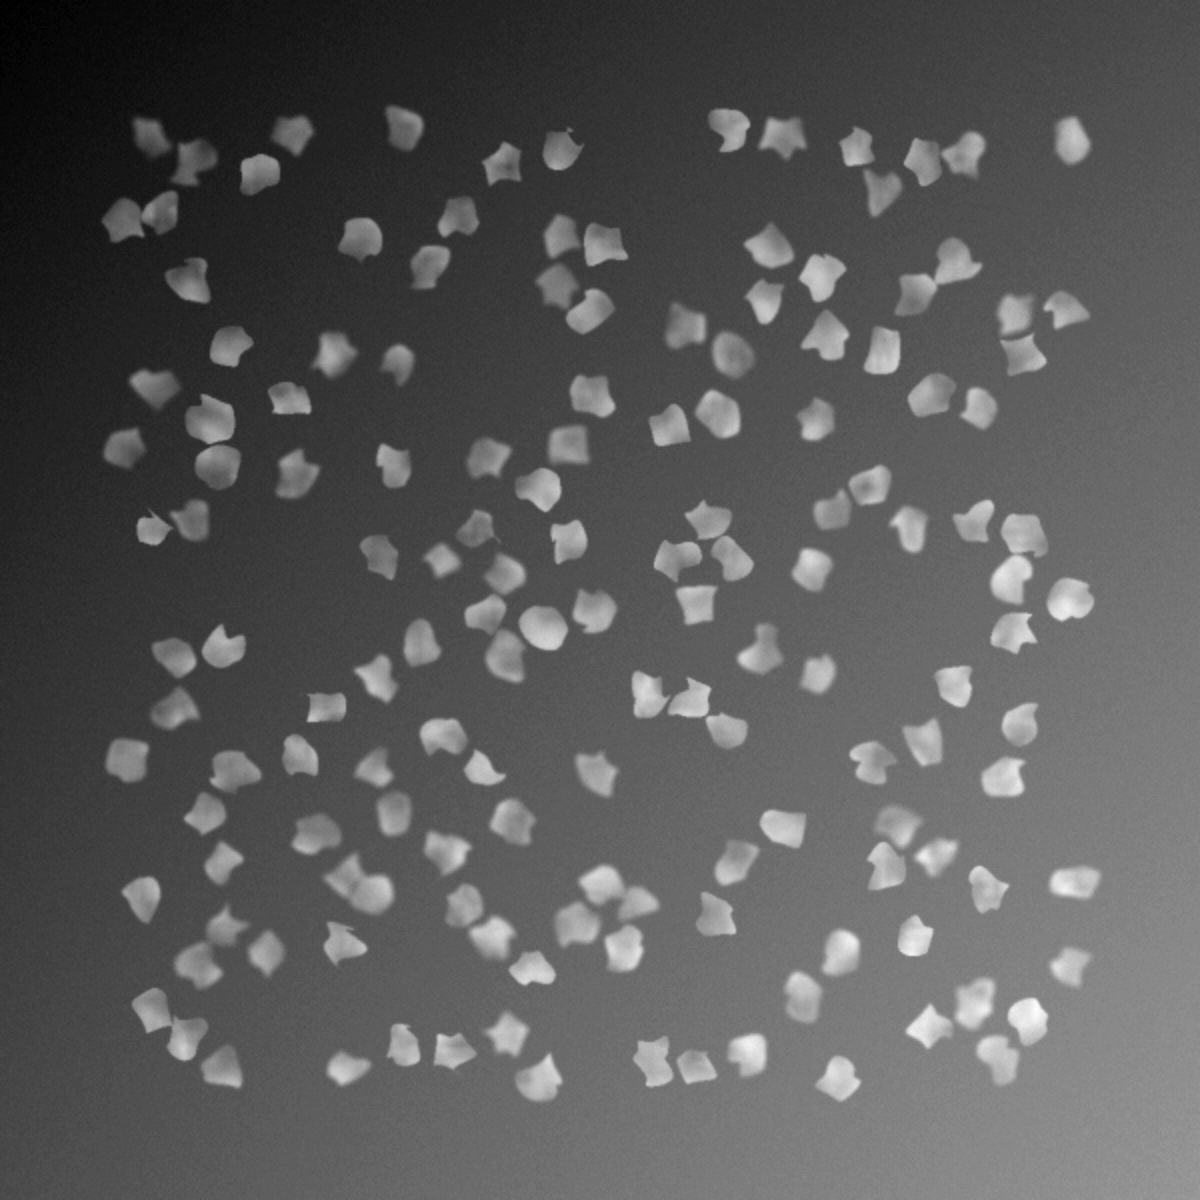
\includegraphics[width=0.3\linewidth]{cells.png}
%     \caption{Useful figure}
%     \label{fig:figurecell}
% \end{figure}


% \todo{Give an overview of the project.}

% \todo{Answer questions from Website Chapter 1.3}

% \todo{Motivate the project for medical approaches}

% Figure \ref{fig:figurecell} shows ...
\section{Introduction}%
\label{sec:introduction}

% All images are defined here
\begin{figure}
    \centering
    \includegraphics[width=0.3\linewidth]{\imagedir cells.png}
    \caption{Cells Original Image}
    \label{fig:figurecell}
\end{figure}


In this project, we undertook various image processing and thresholding tasks, all aimed at enhancing the clarity and visibility of images for easier analysis and interpretation. These tasks are crucial in the field of medical imaging, where the ability to accurately segment and highlight specific regions within an image can significantly impact diagnosis and treatment planning. By leveraging different mathematical formulas and processing techniques, our goal was to produce images with sharp edges and clear distinctions between different elements, making them more informative and easier to analyze.

The advancements in techniques and high-level computing have made it possible to perform intricate image processing tasks at the pixel level, delivering results in a matter of seconds. This capability is particularly important in medical fields, such as oncology, where imaging techniques are used to diagnose conditions at the cellular level. Besides cancer diagnosis, image processing techniques are also widely used in areas such as radiology, cardiology, ophthalmology, and pathology, where clear and accurate imaging is critical for patient care.

Figure \ref{fig:figurecell} displays the original 8-bit grayscale cellular image used throughout this project. Various processing techniques will be applied to this image, and the resulting images will be discussed and analyzed.

The overview of this project is that we complete a range of image processing and thresholding tasks, starting with basic thresholding and moving through to more complex techniques like edge detection. These tasks were designed to build a comprehensive understanding of how different image processing methods can be applied to enhance image quality and segment specific regions of interest.

For instance, basic thresholding was used to convert grayscale images into binary images by setting a threshold value, while more advanced techniques like Otsu’s method were applied to automatically determine the optimal threshold for images with the help of histograms. Edge detection techniques were also implemented to identify the boundaries of objects within images, providing a clear visual distinction between different elements.

Questions from the chapter require that thresholding is a fundamental technique in image processing that converts grayscale images into binary images by setting a threshold value. This method is widely used for its simplicity and efficiency, particularly in scenarios that require quick segmentation of images. Compared to methods like edge detection, which focuses on identifying the boundaries within an image, thresholding is a more straightforward approach that assigns pixel values based on their intensity relative to the threshold.

If we compare thresholding with other techniques, While it is effective for simple segmentation tasks, more complex images might require advanced techniques. For example, adaptive thresholding adjusts the threshold value based on local pixel intensity, making it more suitable for images with varying illumination. Otsu's method, on the other hand, is particularly useful for images with bimodal histograms, as it automatically finds the threshold that maximizes the variance between the two classes.

In contrast to these thresholding methods, edge detection techniques like the Sobel, SCharr, Prewitt, and Canny are designed to detect the edges of objects within an image. These methods are often used in conjunction with thresholding to refine the segmentation process. For example, Canny edge detection provides a more refined edge map by considering gradients in the image, making it more robust against noise compared to basic thresholding.

When it comes to image segmentation, methods like region-based segmentation or deep learning-based approaches (e.g., UNet) offer higher accuracy but at the cost of increased computational resources and complexity. These methods are generally used in situations where the quality of segmentation is critical, such as in medical image analysis for detecting tumors or other abnormalities.


The primary motivation for this project is to enhance the clarity and visibility of images in medical contexts, where accurate imaging is essential for diagnosing and treating diseases. By using optimal image processing techniques, we can improve the quality of images, making them clearer and more informative for medical professionals.

For example, in cancer diagnosis, where imaging at the cellular level is required, the ability to distinguish between healthy and abnormal cells can be greatly enhanced through advanced thresholding and segmentation techniques. This not only aids in diagnosis but also in monitoring the progression of the disease and evaluating the effectiveness of treatments.

Moreover, image processing is not limited to medical applications. It is widely used in various fields such as satellite imaging, industrial quality control, and security systems, where the ability to process and analyze images accurately is crucial. By understanding and applying different image processing techniques, we can develop customized solutions that meet the specific needs of each application, ultimately leading to better outcomes and more informed decision-making.

% \section{Method}
% \subsection{Thresholding and Illumination-Correction}
% \todo{Answer questions about Chapter 1.4}

\section{Method Implementation}
\subsection{Thresholding and Illumination-Correction}

In this project, we implemented three methods: \textbf{run}, \textbf{correctIllumination}, and \textbf{threshold}. Each of these methods plays a vital role in processing the image, correcting uneven illumination, and applying thresholding to generate a binary image.

\textbf{run} serves as the main entry point for processing the image. When the method is executed, a dialog box appears allowing the user to specify a threshold value and choose whether to correct uneven illumination. If the dialog is canceled, no further processing occurs, and the original image is simply displayed.

If the option to correct uneven illumination is selected, the \textbf{correctIllumination} method is invoked. This method is responsible for normalizing the lighting across the image, which is particularly useful in microscopy where uneven illumination can obscure important details. After correcting the illumination (if selected), the \textbf{threshold} method is applied to create a binary image based on the specified threshold value.

The \textbf{correctIllumination} method is designed to normalize uneven lighting in an image. This is achieved by applying a Gaussian blur, a process that smooths the image by averaging the pixel values with their neighbors, weighted by a Gaussian function. The Gaussian blur helps to isolate and remove gradual variations in illumination, resulting in a more uniform background.

\textbf{Gaussian Blur:} Gaussian blur is a low-pass filter that reduces the high-frequency components in the image, making the image appear smoother. The degree of blurring is controlled by the \textit{sigma} value, which determines the spread of the Gaussian function. A higher \textit{sigma} value results in more extensive blurring. When the Gaussian blur is applied, the blurred image is then divided by the original image to correct the illumination.

In the figures below, you can observe the effects of applying Gaussian blur with different \textit{sigma} values. Figure \ref{fig:figure50gaussianblur} shows the image with \textit{sigma} set to 50, Figure \ref{fig:figure75gaussianblur} with \textit{sigma} at 75, and Figure \ref{fig:figure100gaussianblur} with \textit{sigma} at 100. As the \textit{sigma} value increases, the image becomes progressively smoother, highlighting the importance of choosing an appropriate \textit{sigma} value for effective illumination correction.

\begin{figure}[h!]
    \centering
    \begin{subfigure}{0.3\linewidth}
        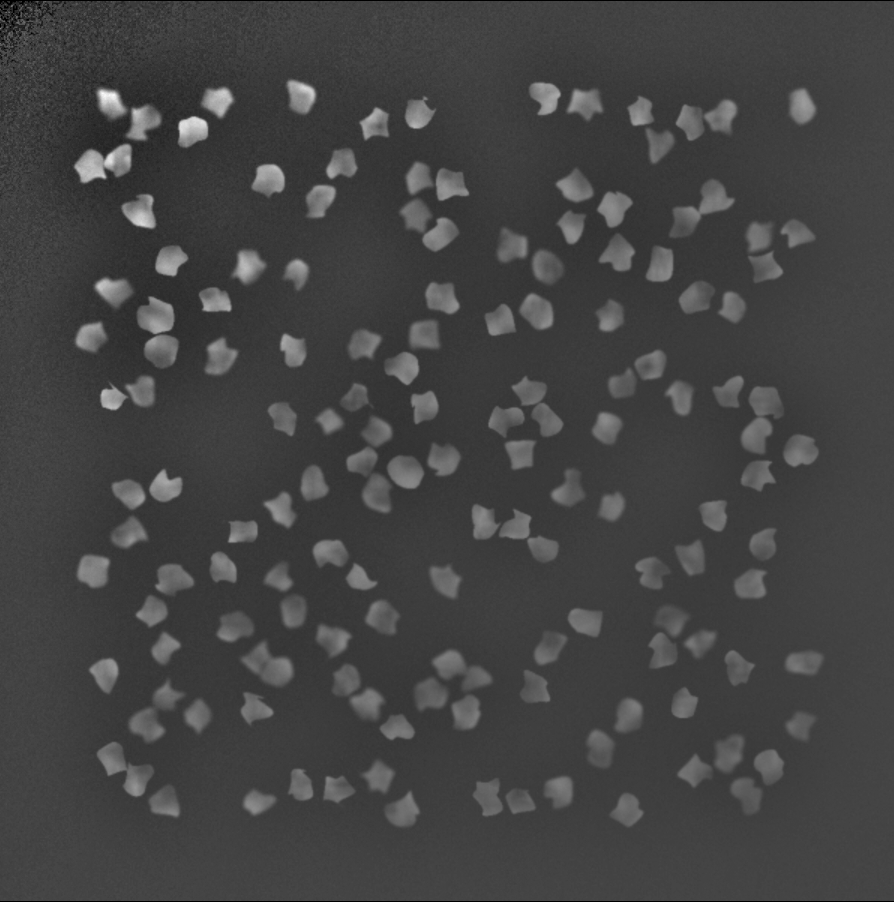
\includegraphics[width=\linewidth]{latex-template-ss24/images/50_Gaussian_blur.png}
        \caption{Sigma Value 50}
        \label{fig:figure50gaussianblur}
    \end{subfigure}
    \begin{subfigure}{0.3\linewidth}
        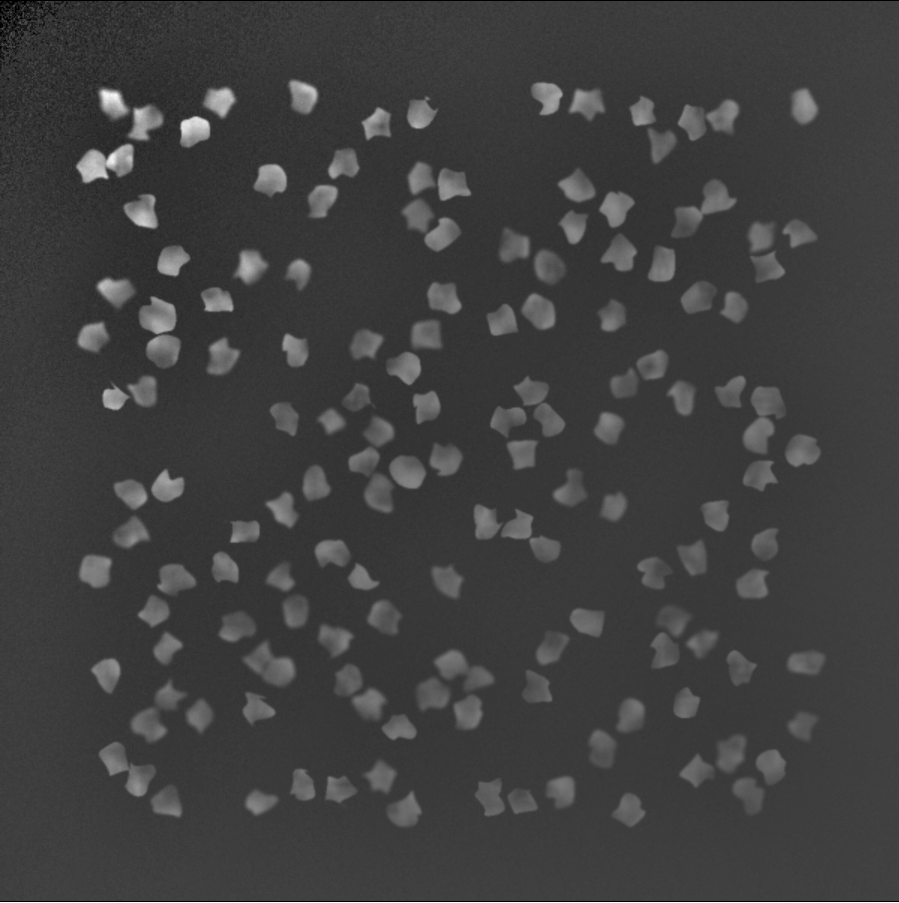
\includegraphics[width=\linewidth]{latex-template-ss24/images/75_Gaussian_blur.png}
        \caption{Sigma Value 75}
        \label{fig:figure75gaussianblur}
    \end{subfigure}
    \begin{subfigure}{0.3\linewidth}
        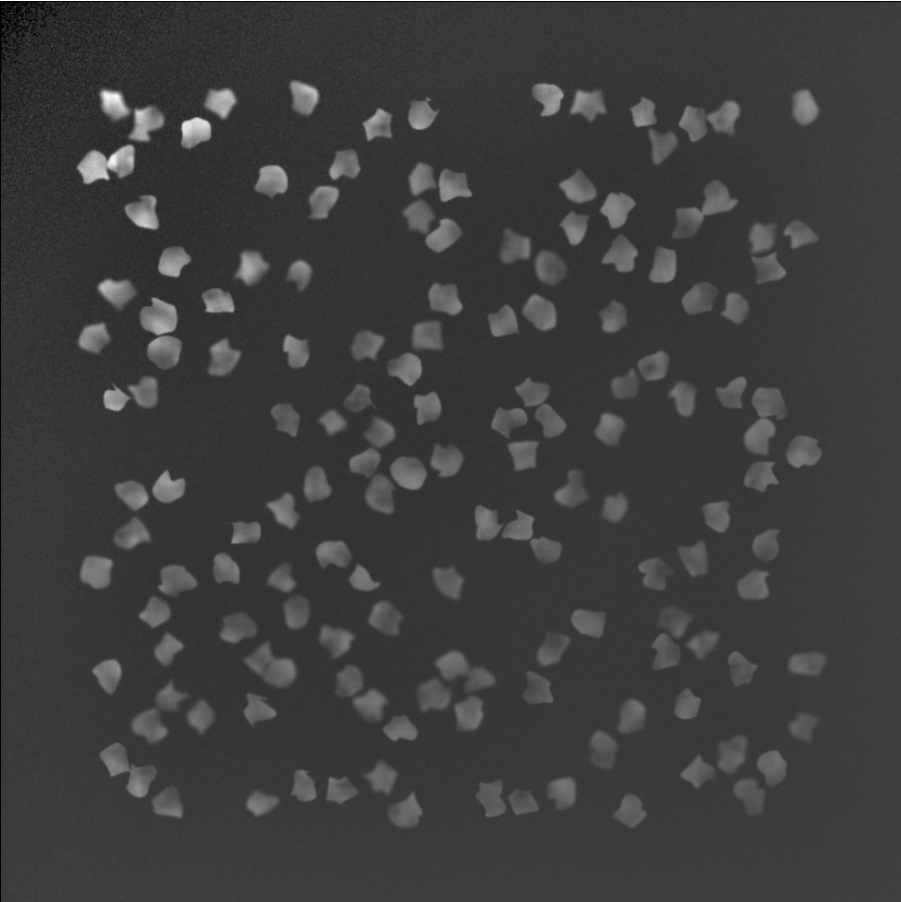
\includegraphics[width=\linewidth]{latex-template-ss24/images/100_Gaussian_blur.png}
        \caption{Sigma Value 100}
        \label{fig:figure100gaussianblur}
    \end{subfigure}
    \caption{Comparison of Gaussian Blur with different Sigma values.}
    \label{fig:gaussian_blur_comparison}
\end{figure}


The \textbf{threshold} method is responsible for converting the grayscale image into a binary image. This is done by setting a threshold value: pixels with intensity values greater than the threshold are set to white, while those with lower values are set to black. This process effectively segments the image into two distinct regions, making it easier to analyze specific features.

In Figure \ref{fig:figure128thresholding}, you can see the results of applying thresholding with the default value of 128.0. The resulting image is a clear binary representation of the original image. When the threshold value is increased to 200, as shown in Figure \ref{fig:figure200thresholding}, more of the image turns black because a larger number of pixels in the original image have intensity values below 200.

% Placeholder for image insertion
% Insert Figures 5 and 6 here
\begin{figure}[h!]
    \centering
    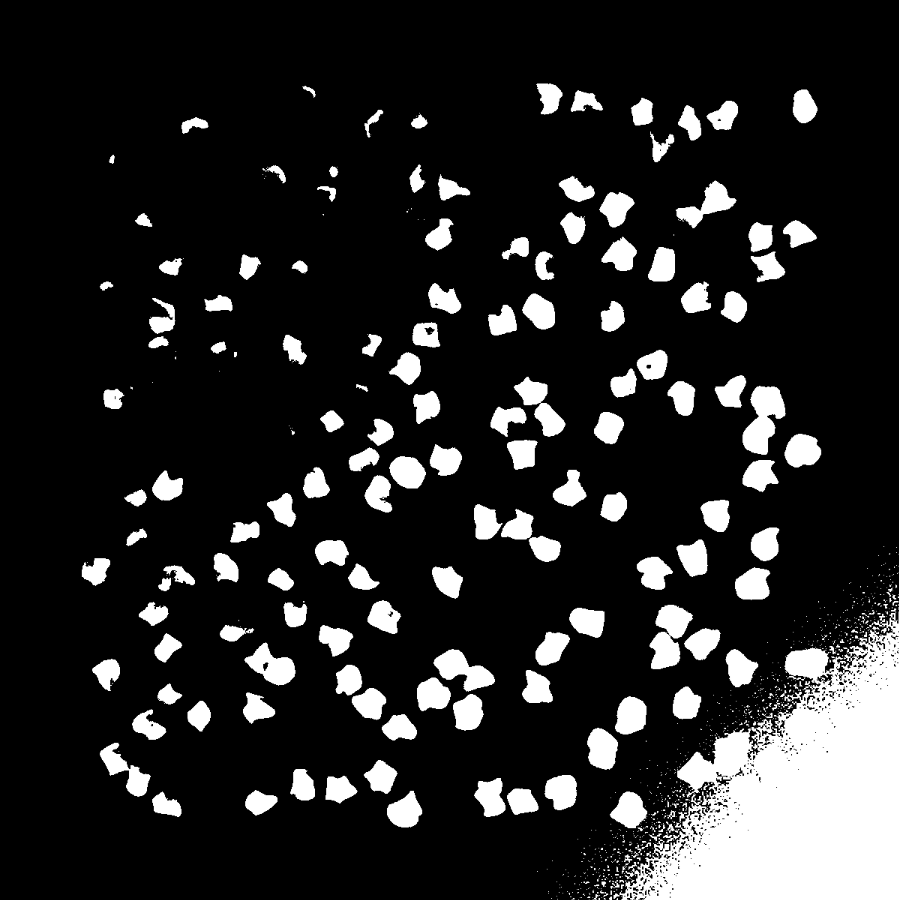
\includegraphics[width=0.3\linewidth]{latex-template-ss24/images/128_threshold.png}
    \caption{Thresholding at Value 128}
    \label{fig:figure128thresholding}
\end{figure}

\begin{figure}[h!]
    \centering
    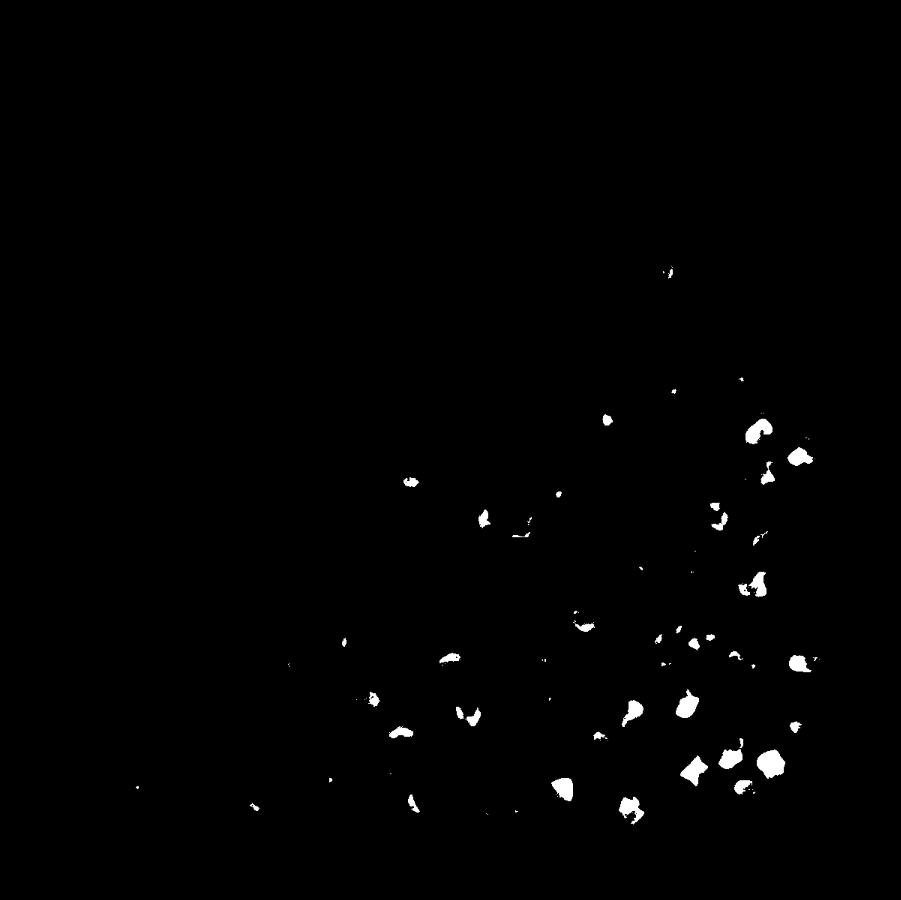
\includegraphics[width=0.3\linewidth]{latex-template-ss24/images/200_threshold.png}
    \caption{Thresholding at Value 200}
    \label{fig:figure200thresholding}
\end{figure}

Correcting illumination in microscopy images is often necessary to ensure accurate analysis and interpretation. Uneven illumination can introduce artifacts and distortions, leading to potential misinterpretations of the microscopic structures. These issues are particularly problematic when precise details, such as the boundaries of cells or tissues, need to be clearly visualized.

In microscopy, uneven illumination can result from several factors, including the light source's intensity distribution, the microscope optics, and the specimen's geometry. Correcting these inconsistencies is essential to achieving a more uniform image, where the true structures are more apparent and not masked by lighting artifacts. This correction process is crucial for tasks such as image segmentation, where accurate differentiation between regions based on intensity values is necessary. Without proper illumination correction, these regions may be incorrectly identified, leading to inaccurate results \cite{leong2003correction}. Moreover, reducing illumination-related artifacts is vital to ensure that quantitative analyses accurately reflect the specimen's characteristics, free from distortions caused by uneven lighting.

By applying the `correctIllumination` method before thresholding, we reduce the noise and enhance the contrast between the structures of interest and the background. This step is particularly beneficial in cases where the biological structures are faint and could otherwise be lost in the unevenly illuminated regions of the image. As a result, the corrected images are more reliable and provide a better foundation for subsequent image processing tasks, such as segmentation or quantitative analysis. 

An optimal threshold value of 88 was determined and applied, yielding the most accurate results after correcting the image as show in Figure \ref{fig:figure88thresholding}. The method for achieving this optimal threshold value will be discussed in subsequent sections.
 

% Placeholder for image insertion
% Insert final comparison images here


\begin{figure}[h!]
    \centering
    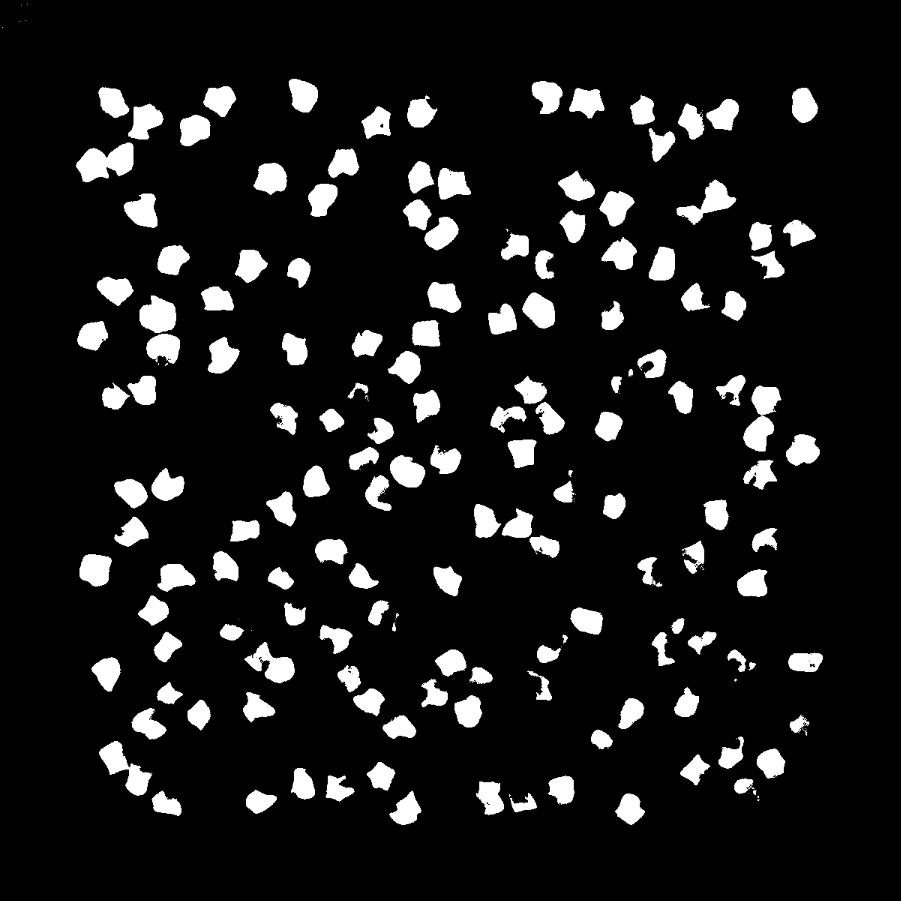
\includegraphics[width=0.3\linewidth]{latex-template-ss24/images/88_thresholded_corrected_illumination.png}
    \caption{Thresholding at Value 88}
    \label{fig:figure88thresholding}
\end{figure}


% \subsection{Image Segmentation}
% \todo{Answer questions about Chapter 2}

% \todo{Provide the formulas for Specificity and Sensitivity.}
% \begin{equation}
%     Specificity =  \\
% \end{equation}
% \begin{equation} 
%     Sensitivity = \\
% \end{equation}
\subsection{Image Segmentation}
In this task, we performed segmentation of the image. Image segmentation is the process of dividing an image into multiple segments or regions to simplify or change the representation of the image into something more meaningful and easier to analyze. It is a crucial step in image processing and computer vision, particularly for identifying and delineating objects or regions of interest in an image.

In the context of medical imaging, segmentation helps in identifying various structures such as tissues, organs, or abnormal regions like tumors. The performance of a segmentation algorithm can be assessed using various metrics, including True Positives (TP), True Negatives (TN), False Positives (FP), and False Negatives (FN), which are defined as follows:

- \textbf{True Positive (TP)}: The number of pixels correctly identified as part of the object of interest.
- \textbf{True Negative (TN)}: The number of pixels correctly identified as not part of the object of interest.
- \textbf{False Positive (FP)}: The number of pixels incorrectly identified as part of the object of interest.
- \textbf{False Negative (FN)}: The number of pixels incorrectly identified as not part of the object of interest.

Specificity and Sensitivity are key metrics used to evaluate the performance of the segmentation:

\textbf{Specificity} is defined as the proportion of true negatives out of the total number of actual negatives:
\begin{equation}
    \text{Specificity} = \frac{TN}{TN + FP}
\end{equation}

\textbf{Sensitivity} is defined as the proportion of true positives out of the total number of actual positives:
\begin{equation}
    \text{Sensitivity} = \frac{TP}{TP + FN}
\end{equation}

Both metrics are crucial in evaluating the performance of a segmentation method. High sensitivity indicates that the method is good at identifying the object of interest, while high specificity means that the method is effective at distinguishing the object from the background.

We performed segmentation on six thresholded images as seen in the figures below. The top row shows images without illumination correction, while the bottom row shows images with illumination correction. The threshold values used are 128, 200, and 88.

\begin{figure}[H]
    \centering
    \begin{subfigure}{0.3\linewidth}
        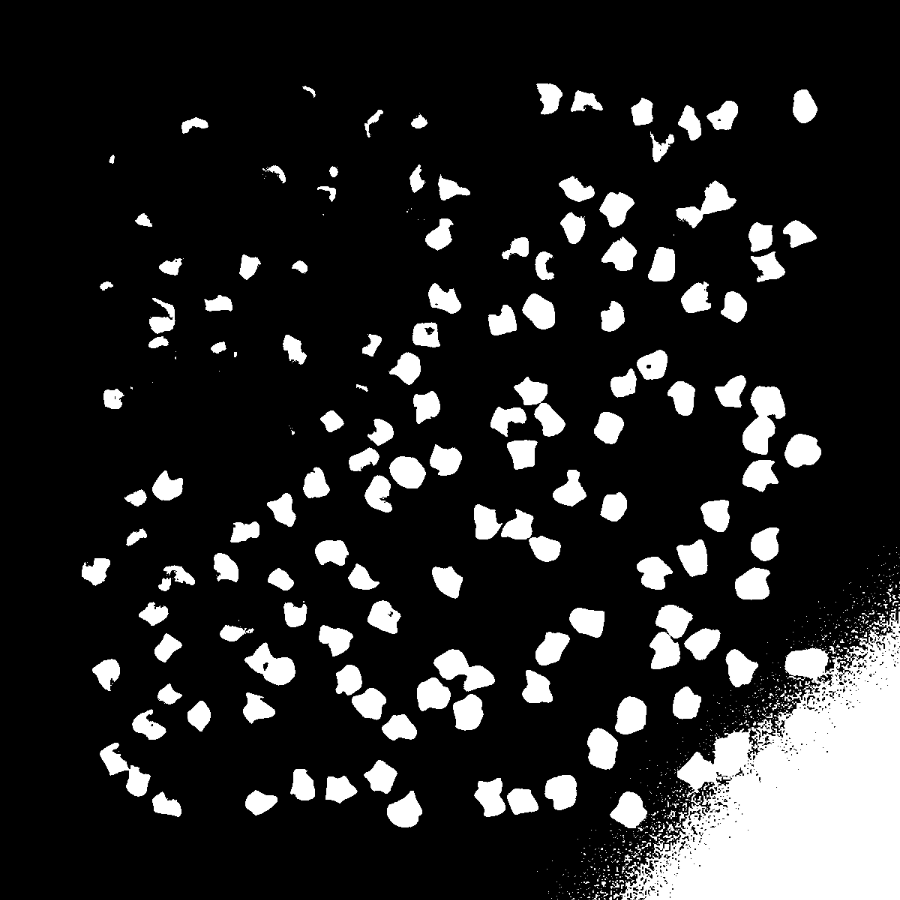
\includegraphics[width=\linewidth]{latex-template-ss24/images/segmentation_128_threshold_non_illuminated.png}
        \caption{Threshold 128, Non-Illuminated}
        \label{fig:segmentation_128_threshold_non_illuminated}
    \end{subfigure}
    \begin{subfigure}{0.3\linewidth}
        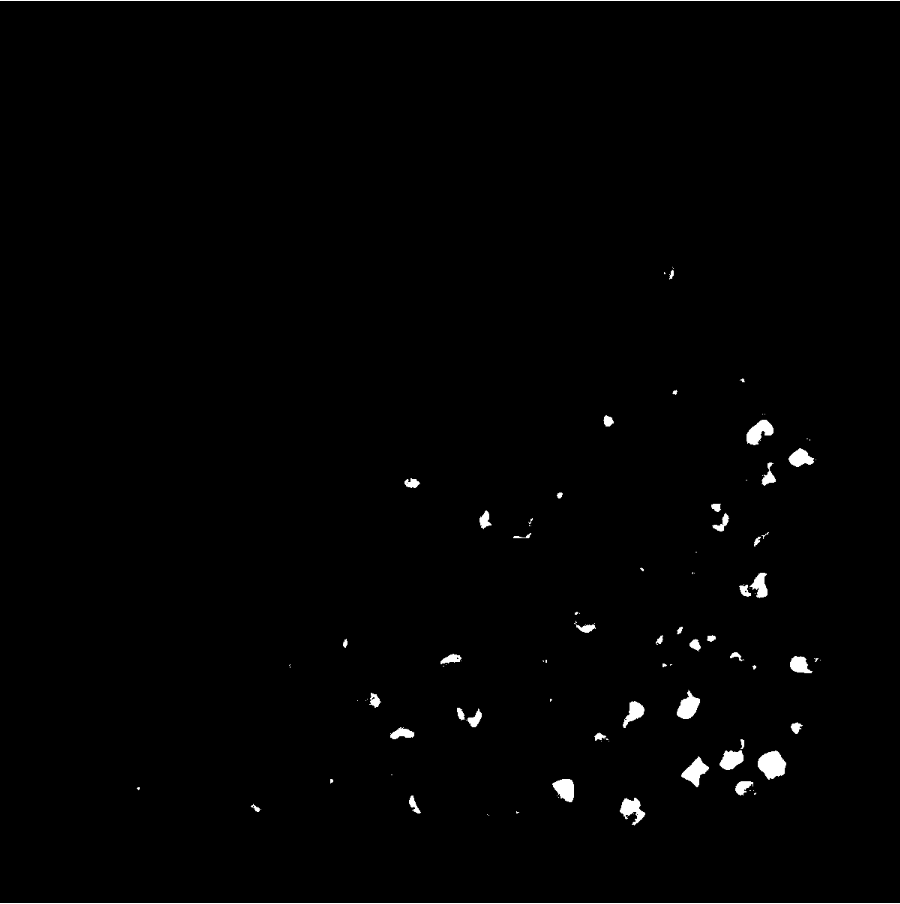
\includegraphics[width=\linewidth]{latex-template-ss24/images/segmentation_200_threshold_non_illuminated.png}
        \caption{Threshold 200, Non-Illuminated}
        \label{fig:segmentation_200_threshold_non_illuminated}
    \end{subfigure}
    \begin{subfigure}{0.3\linewidth}
        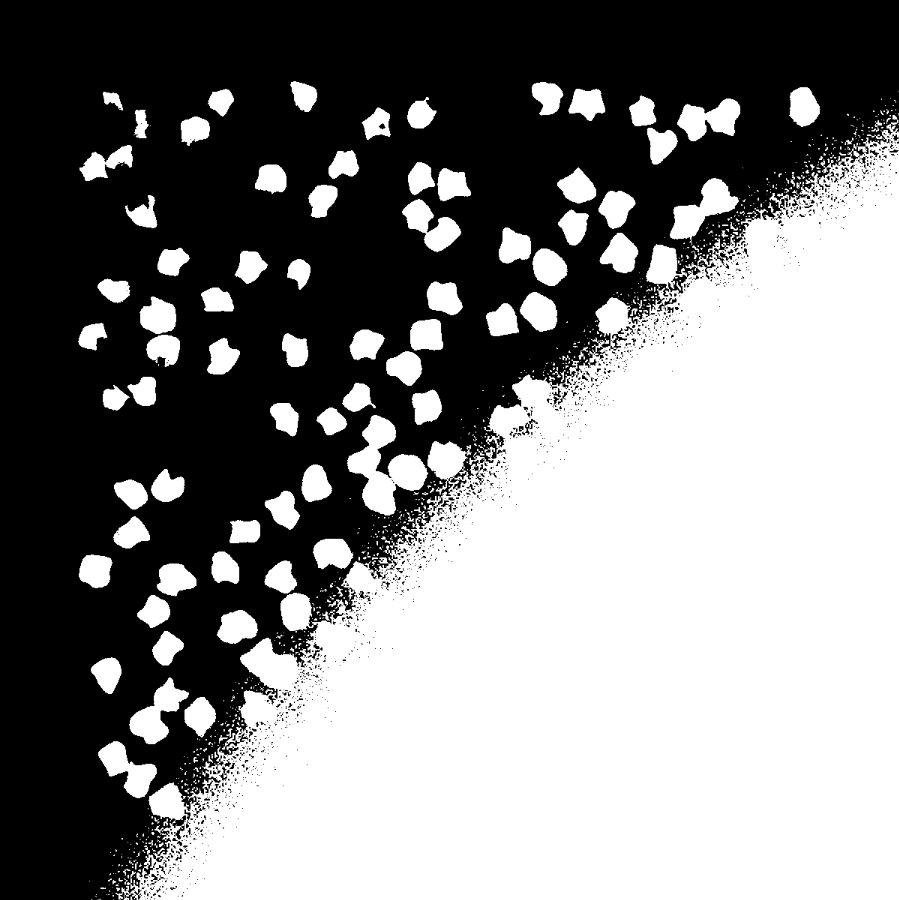
\includegraphics[width=\linewidth]{latex-template-ss24/images/segmentation_88_threshold_non_illuminated.png}
        \caption{Threshold 88, Non-Illuminated}
        \label{fig:segmentation_88_threshold_non_illuminated}
    \end{subfigure}
    
    \begin{subfigure}{0.3\linewidth}
        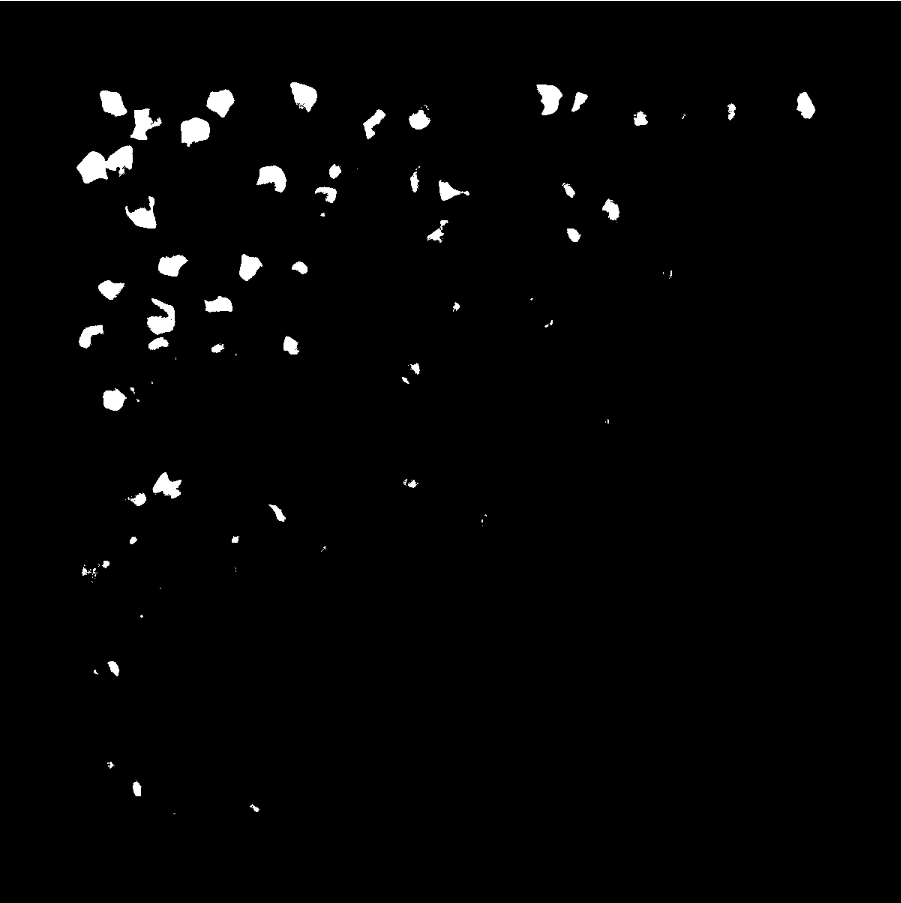
\includegraphics[width=\linewidth]{latex-template-ss24/images/segmentation_128_threshold_illuminated.png}
        \caption{Threshold 128, Illuminated}
        \label{fig:segmentation_128_threshold_illuminated}
    \end{subfigure}
    \begin{subfigure}{0.3\linewidth}
        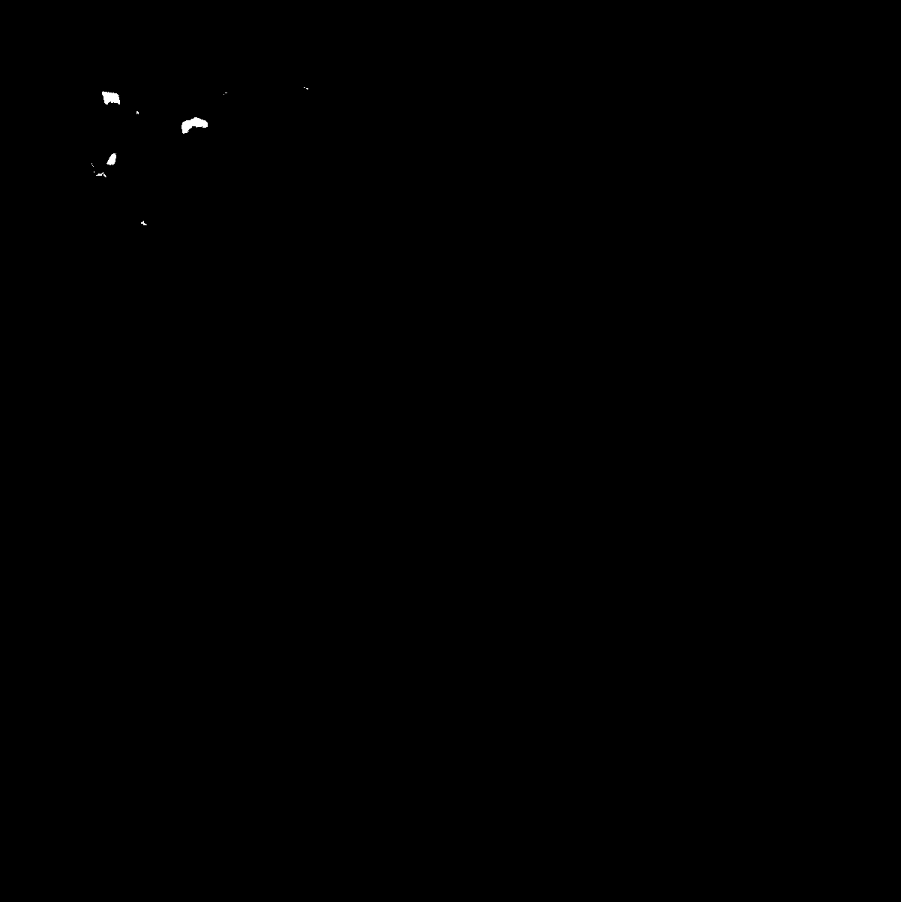
\includegraphics[width=\linewidth]{latex-template-ss24/images/segmentation_200_threshold_illuminated.png}
        \caption{Threshold 200, Illuminated}
        \label{fig:segmentation_200_threshold_illuminated}
    \end{subfigure}
    \begin{subfigure}{0.3\linewidth}
        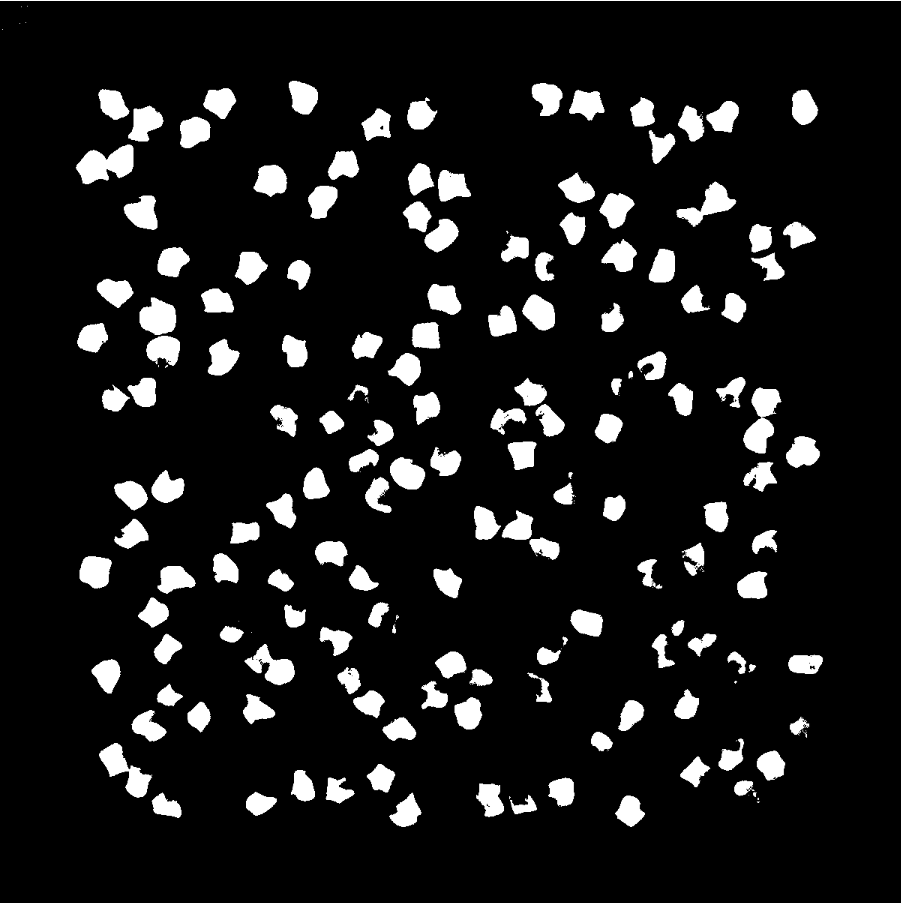
\includegraphics[width=\linewidth]{latex-template-ss24/images/segmentation_88_threshold_illuminated.png}
        \caption{Threshold 88, Illuminated}
        \label{fig:segmentation_88_threshold_illuminated}
    \end{subfigure}
    
    \caption{Comparison of thresholding with and without illumination correction. Top row: non-illuminated, bottom row: illuminated.}
    \label{fig:segmentation_comparison}
\end{figure}

The segmentation results highlight the impact of illumination correction. Without illumination correction, the segmentation is less accurate, especially in regions with varying brightness. After applying illumination correction, the segmentation becomes more reliable, with better sensitivity and specificity metrics. 

\textbf{Additional Methods for Evaluating Segmentation}, apart from sensitivity and specificity, two other methods for evaluating segmentation include:

- \textbf{Dice Coefficient}: The Dice Coefficient, also known as the Sørensen-Dice index, is a statistical measure used to evaluate the similarity between two samples. In the context of image segmentation, it quantifies the overlap between the predicted segmentation and the ground truth segmentation. The Dice Coefficient ranges from 0 (no overlap) to 1 (perfect overlap) and is computed as follows:

  \[
  \text{Dice Coefficient} = \frac{2 \times TP}{2 \times TP + FP + FN}
  \]

  The Dice Coefficient is particularly useful in medical imaging where accurate segmentation is critical, such as in tumor detection or organ delineation \cite{zou2004statistical}.

- \textbf{Jaccard Index (Intersection over Union)}: The Jaccard Index, also known as Intersection over Union (IoU), measures the similarity between two sets by comparing their intersection and union. In image segmentation, it is calculated as:

  \[
  \text{Jaccard Index} = \frac{TP}{TP + FP + FN}
  \]

  The Jaccard Index is a more stringent measure than the Dice Coefficient, providing a robust evaluation by accounting for both false positives and false negatives \cite{real1996probabilistic}.

% \subsection{Otsu's Method}
% \todo{Cite \cite{Otsu}}

% \todo{Answer questions about Chapter 3}
% As mentioned in Section \ref{sec:introduction}. 

\subsection{Otsu's Method}

Otsu's method is a statistical technique used in image segmentation to automatically determine the optimal threshold value that separates the foreground and background of a grayscale image. The method aims to minimize the variance within each class (foreground and background) while maximizing the variance between the classes. This ensures that the threshold selected is optimal for distinguishing between the two regions.

Mathematically, Otsu's method works as follows:

1. \textbf{Histogram Calculation}: The histogram of the image is computed to represent the frequency of each intensity level.

2. \textbf{Probability Distributions}: The cumulative probability distributions for the foreground (\(P1(\theta)\)) and background (\(P2(\theta)\)) are computed based on the histogram.

3. \textbf{Mean Intensities}: The mean intensity values for the foreground (\(\mu1(\theta)\)) and background (\(\mu2(\theta)\)) are calculated.

4. \textbf{Between-Class Variance}: The between-class variance (\(\sigma_B^2(\theta)\)) is then computed, which quantifies the separation between the two classes. The threshold that maximizes this variance is selected as the optimal threshold.

Otsu's method is particularly effective for images with a bimodal histogram, where the pixel intensities can be clearly divided into two distinct groups. However, it has limitations, including its sensitivity to noise and its assumption of a bimodal histogram, which may not hold for all images.

In the original publication, Otsu emphasizes that "An optimal threshold is selected automatically and stably, not based on the differentiation (i.e., a local property such as valley), but on the integration (i.e., a global property) of the histogram." This means that Otsu's method considers the overall distribution of pixel intensities in the image, rather than focusing on local minima or other local features in the histogram. The "integration" refers to the method's use of cumulative distributions to evaluate the histogram as a whole, ensuring that the thresholding decision is based on global properties rather than local fluctuations \cite{Otsu1979}.

If we do comparison with Naive thresholding methods typically involve selecting a threshold value based on simple criteria, such as the midpoint between the minimum and maximum intensity values in the image. While straightforward, this approach can be ineffective for images with complex intensity distributions, as it does not account for the distribution of pixel values across the image. Otsu's method, on the other hand, evaluates the entire histogram and finds a threshold that optimally separates the foreground and background based on statistical properties, making it more robust in many scenarios.

Talking about limitations and modern alternatives despite its effectiveness, Otsu's method has several shortcomings. First, it assumes that the image has a bimodal histogram, which may not be true for all images. In cases where the histogram is unimodal or multimodal, the method may fail to find an optimal threshold. Second, Otsu's method is sensitive to noise, which can distort the histogram and lead to suboptimal threshold selection.

To address these issues, modern methods such as adaptive thresholding and deep learning-based approaches have been developed. Adaptive thresholding, for instance, adjusts the threshold value for different regions of the image based on local properties, making it more effective in images with varying lighting conditions. Deep learning-based methods, such as those utilizing convolutional neural networks (CNNs), can learn complex patterns and features from the image data, enabling more accurate and robust segmentation in challenging scenarios \cite{Otsu1979, Sezgin2004, Ronneberger2015}.

The segmentation result using Otsu's method on the provided image is shown in Figure \ref{fig:otsu_result}. You can see that it resembles the illuminated image having threshold value 88 from Figure \ref{fig:figure88thresholding}.

\begin{figure}[H]
    \centering
    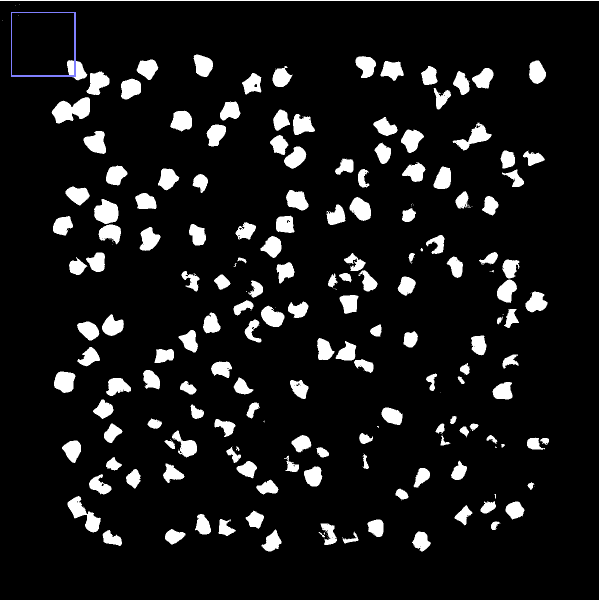
\includegraphics[width=0.3\linewidth]{latex-template-ss24/images/Otsu_image.png}
    \caption{Segmentation result using Otsu's Method}
    \label{fig:otsu_result}
\end{figure}



% \subsection{Edge-detection}
% \todo{Answer questions about Chapter 4}

% \label{sec:edgedetection}

\subsection{Edge-Detection}

\subsection{Edge-Detection}

Edge-detection filters such as Sobel, Scharr, and Prewitt are fundamental techniques used in image processing to identify the boundaries within an image. These filters detect changes in intensity that often correspond to the edges of objects, which are critical for tasks such as object recognition, image segmentation, and computer vision \cite{Gonzalez2008}.

\textbf{Sobel Filter} applies convolution masks to detect changes in intensity in the x-direction (horizontal) and y-direction (vertical). The result is a gradient map that emphasizes edges, particularly those oriented at a 45-degree angle, making it effective for detecting edges aligned with the image axes \cite{Gonzalez2008}. Figure \ref{fig:sobel_edge_detection} below shows the generated image of the Sobel.

\begin{figure}[H]
    \centering
    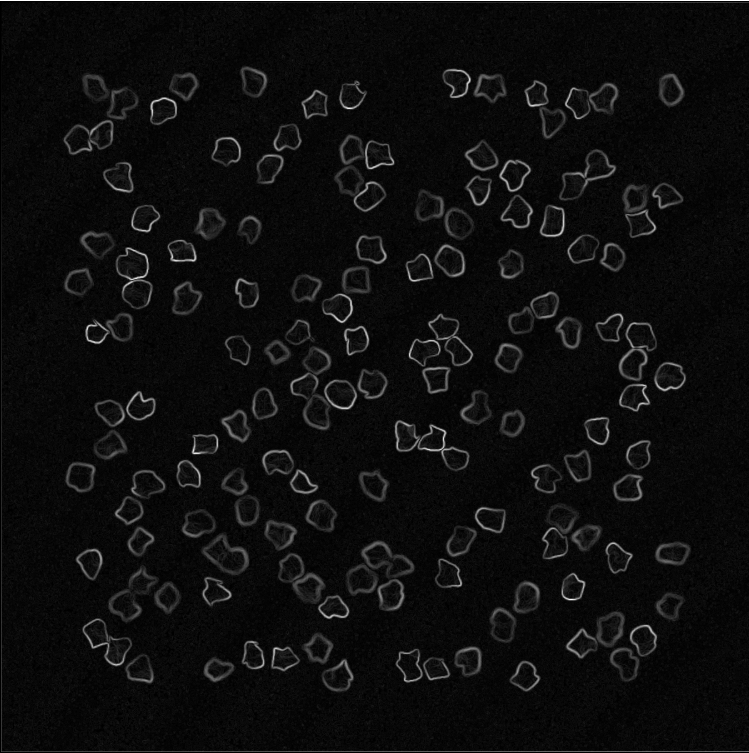
\includegraphics[width=0.3\textwidth]{latex-template-ss24/images/Sobel_edge_detection.png}
    \caption{Sobel Edge Detection}
    \label{fig:sobel_edge_detection}
\end{figure}

\textbf{Scharr Filter}, a refinement of the Sobel operator, provides improved rotational symmetry, which results in more accurate edge detection for edges that are not perfectly aligned with the image axes. Scharr's original work is detailed in his thesis, but for a comprehensive discussion, see the summarization in \cite{Gonzalez2008}. Figure \ref{fig:scharr_edge_detection} below shows the generated image of the Scharr.

\begin{figure}[H]
    \centering
    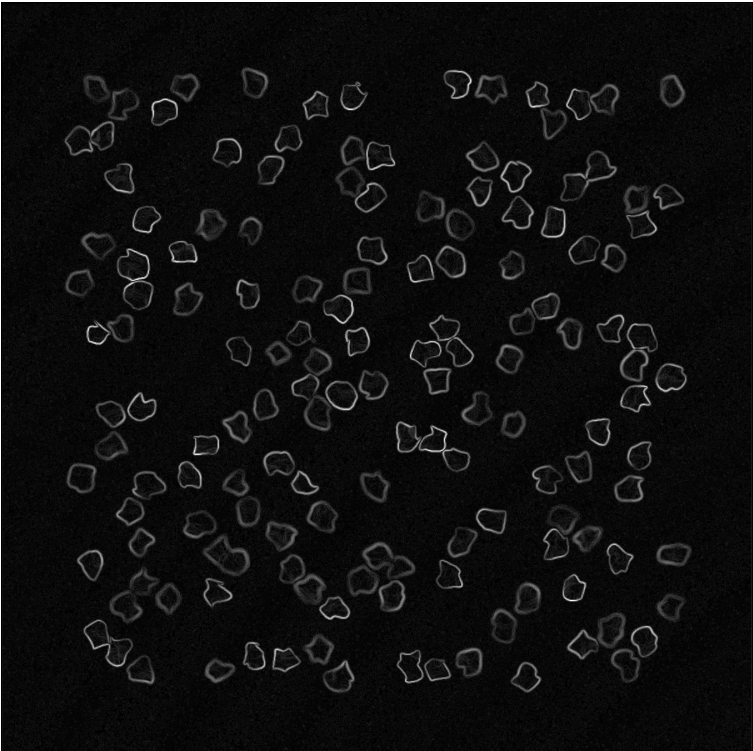
\includegraphics[width=0.3\textwidth]{latex-template-ss24/images/Scharr_edge_detection.png}
    \caption{Scharr Edge Detection}
    \label{fig:scharr_edge_detection}
\end{figure}

\textbf{Prewitt Filter}, similar to the Sobel operator, uses convolution masks to detect horizontal and vertical changes in intensity. While it is simpler and less sensitive to noise compared to the Sobel filter, it is generally less accurate, particularly in detecting diagonal edges \cite{Gonzalez2008}. Figure \ref{fig:prewitt_edge_detection} below shows the generated image of the Prewitt.

\begin{figure}[H]
    \centering
    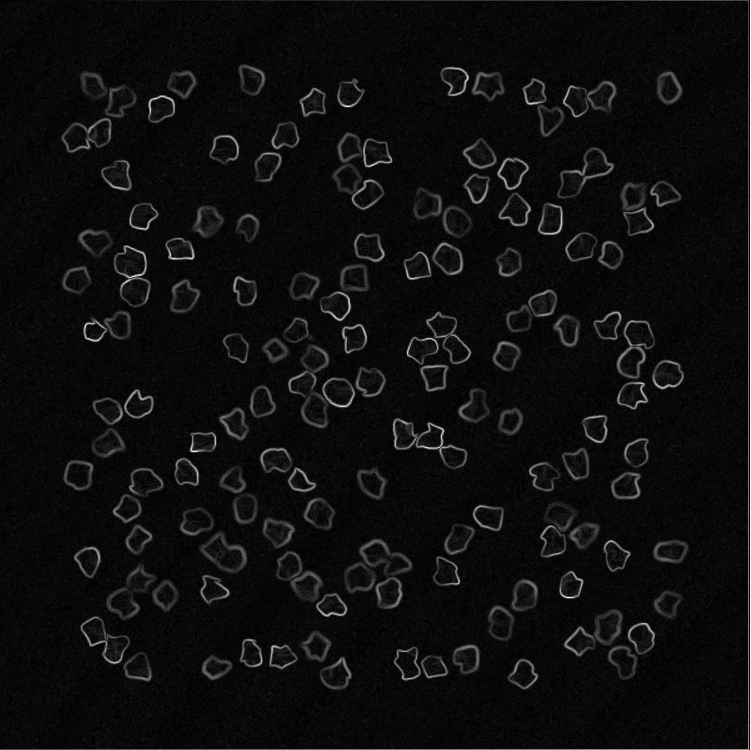
\includegraphics[width=0.3\textwidth]{latex-template-ss24/images/Prewitt_edge_detection.png}
    \caption{Scharr Edge Detection}
    \label{fig:prewitt_edge_detection}
\end{figure}

While effective for basic edge detection tasks, these filters have several limitations:

\begin{itemize}
    \item \textbf{Noise Sensitivity:} These filters are highly sensitive to noise, which can result in false edges, especially in low-contrast or noisy images. Smoothing filters or more advanced methods like Canny edge detection can help mitigate this issue \cite{Canny1986}.
    \item \textbf{Fixed Orientation:} The filters are optimized for detecting edges aligned with the image axes (horizontal and vertical) and may struggle with edges at other orientations. More sophisticated approaches, like the Laplacian of Gaussian or directional filters that consider gradient orientation, can offer better results \cite{Marr1980}.
    \item \textbf{Limited Gradient Information:} These methods consider only the gradient magnitude without accounting for edge orientation or the broader context, limiting their effectiveness in complex scenes. Techniques like the Canny edge detector address this by considering gradient direction and applying non-maximum suppression to refine the edges \cite{Canny1986}.
\end{itemize}


\subsection{Canny Edge Detection}
Canny Edge Detection is a widely used edge detection algorithm developed by John F. Canny in 1986. It aims to detect edges in an image while minimizing the error rate, ensuring accurate edge localization, and providing a single response to edges. The Canny Edge Detector works by applying a Gaussian blur to smooth the image, finding the intensity gradient of the image, applying non-maximum suppression to remove spurious responses, and using double thresholding and edge tracking by hysteresis to detect strong and weak edges.

The Canny Edge Detector is superior to more primitive edge detection methods like Sobel, Scharr, or Prewitt because it includes a noise reduction step (Gaussian blur) and uses two thresholds to differentiate between strong and weak edges, reducing the chances of detecting false edges. Additionally, the non-maximum suppression step helps in achieving thinner and more accurate edges.

The parameters of the Canny Edge Detector significantly influence the results:
\begin{itemize}
    \item \textbf{Sigma (Gaussian Blur):} Controls the amount of smoothing applied to the image before edge detection. A higher sigma value results in more smoothing, which can reduce noise but also cause edge blurring.
    \item \textbf{Upper and Lower Thresholds:} These determine the sensitivity of the edge detection. The upper threshold marks the minimum gradient strength required to consider a pixel as an edge, while the lower threshold allows for the inclusion of connected edges.
\end{itemize}

In the following figures, we observe the impact of varying the parameters of the Canny Edge Detector on the detected edges in the images:

\begin{figure}[H]
    \centering
    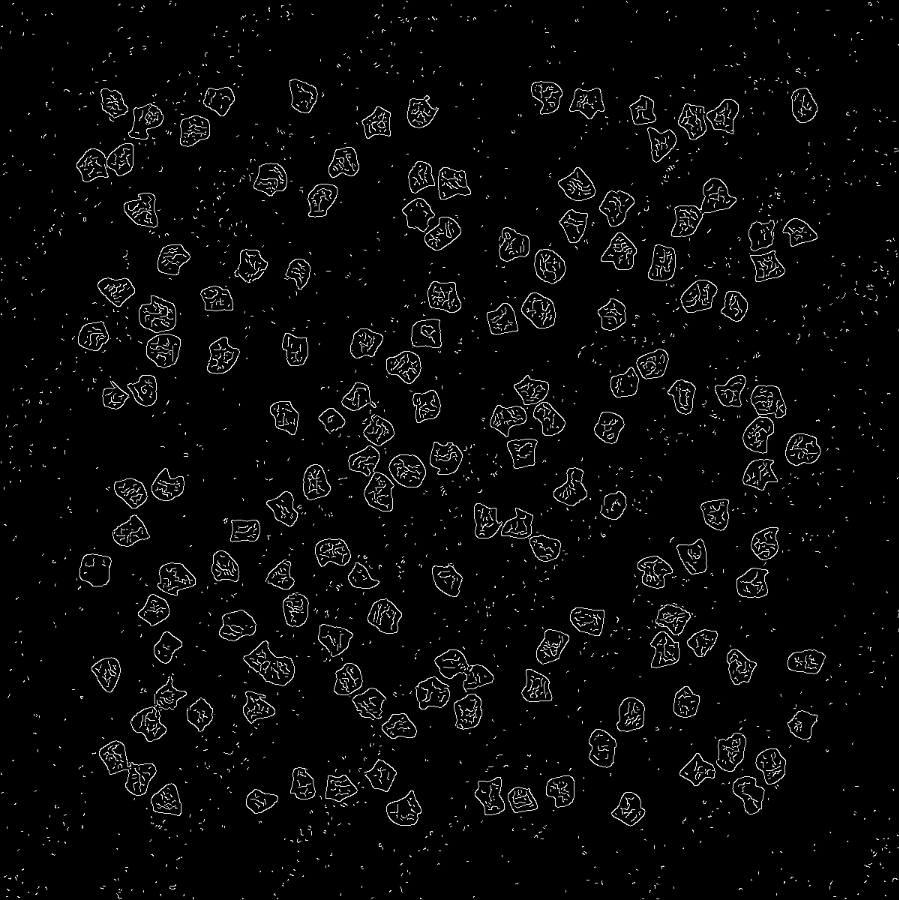
\includegraphics[width=0.3\textwidth]{latex-template-ss24/images/1_15_5_canny.png}
    \caption{Canny Edge Detection with Sigma: 1.0, Upper Threshold: 15\%, Lower Threshold: 5\%}
    \label{fig:1_15_5_canny}
\end{figure}

\textbf{Explanation:} With a low Sigma value of 1.0 and relatively low thresholds (15\% upper and 5\% lower), this configuration results in a detailed edge map where even subtle edges are detected. However, the inclusion of noise and small, irrelevant edges may occur due to the lower thresholds.

\begin{figure}[H]
    \centering
    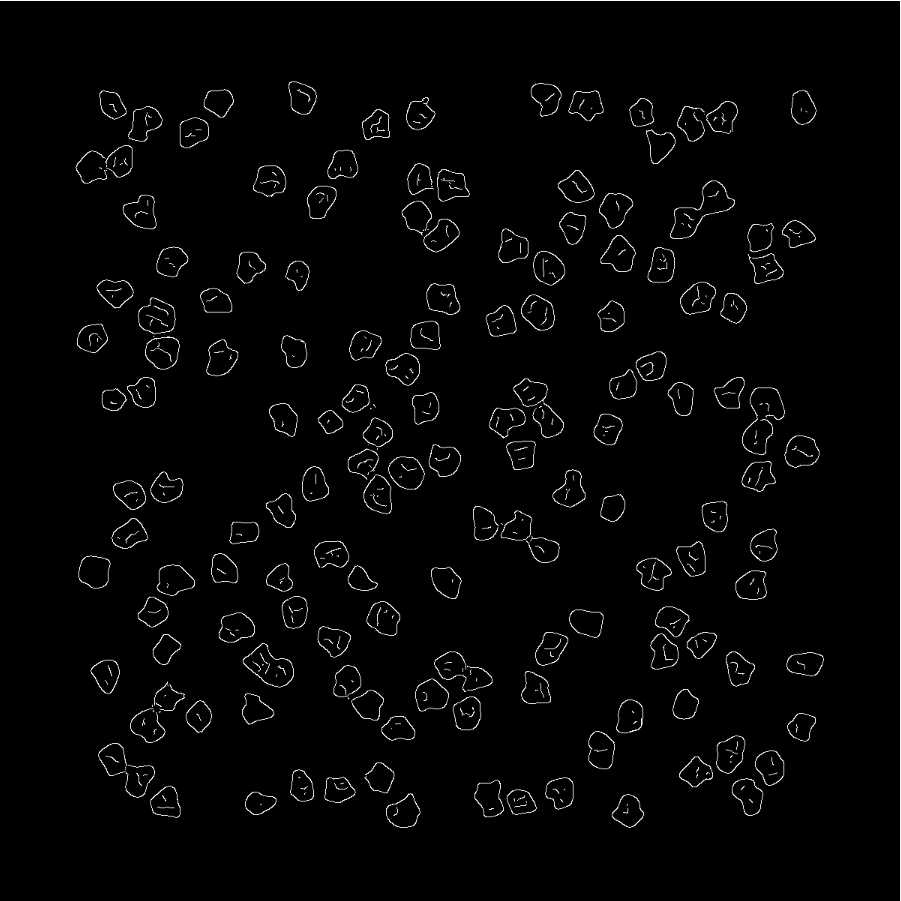
\includegraphics[width=0.3\textwidth]{latex-template-ss24/images/3_25_10_canny.png}
    \caption{Canny Edge Detection with Sigma: 3.0, Upper Threshold: 25\%, Lower Threshold: 10\%}
    \label{fig:3_25_10_canny}
\end{figure}

\textbf{Explanation:} Increasing the Sigma value to 3.0 introduces more smoothing, which reduces noise but also slightly blurs the edges. The higher thresholds (25\% upper and 10\% lower) further filter out weaker edges, leading to a cleaner edge map with fewer detected edges. This configuration is suitable for detecting stronger edges while reducing noise.

\begin{figure}[H]
    \centering
    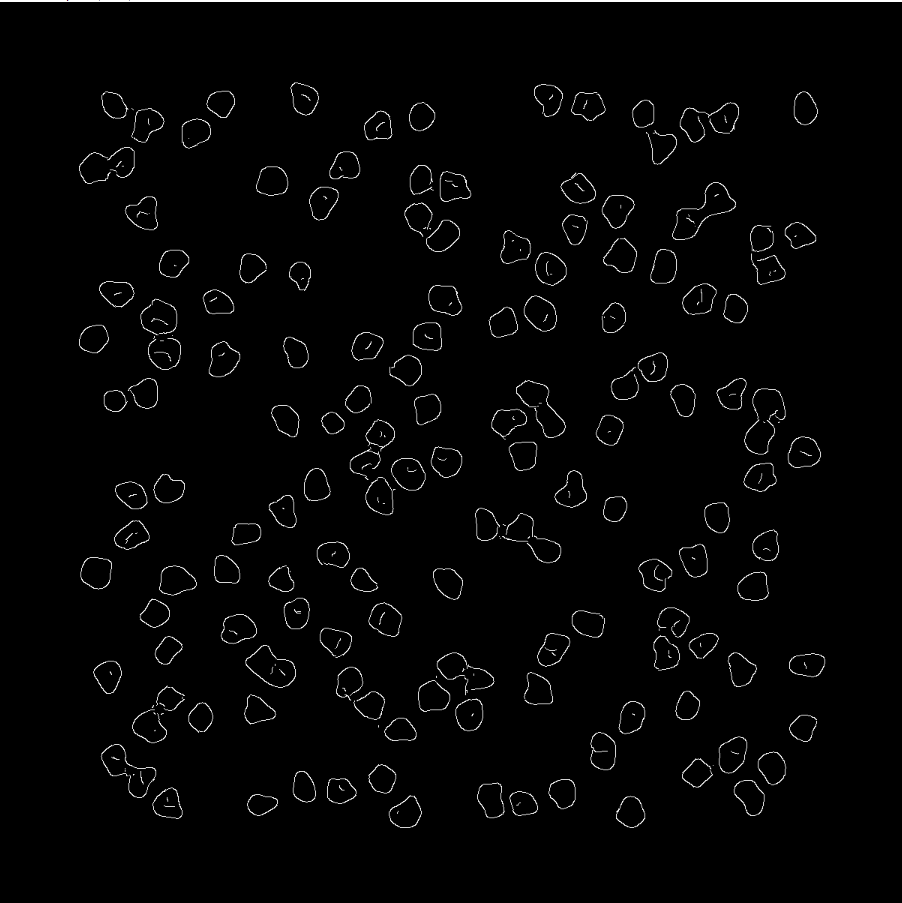
\includegraphics[width=0.3\textwidth]{latex-template-ss24/images/5_30_15_canny.png}
    \caption{Canny Edge Detection with Sigma: 5.0, Upper Threshold: 30\%, Lower Threshold: 15\%}
    \label{fig:5_30_15_canny}
\end{figure}

\textbf{Explanation:} With an even higher Sigma value of 5.0, the image undergoes significant smoothing, which can cause some of the finer edges to be lost. The increased thresholds (30\% upper and 15\% lower) result in a further reduction of detected edges, focusing primarily on the most prominent features. This setup is useful when you want to focus only on the most significant edges in the image.

\begin{figure}[H]
    \centering
    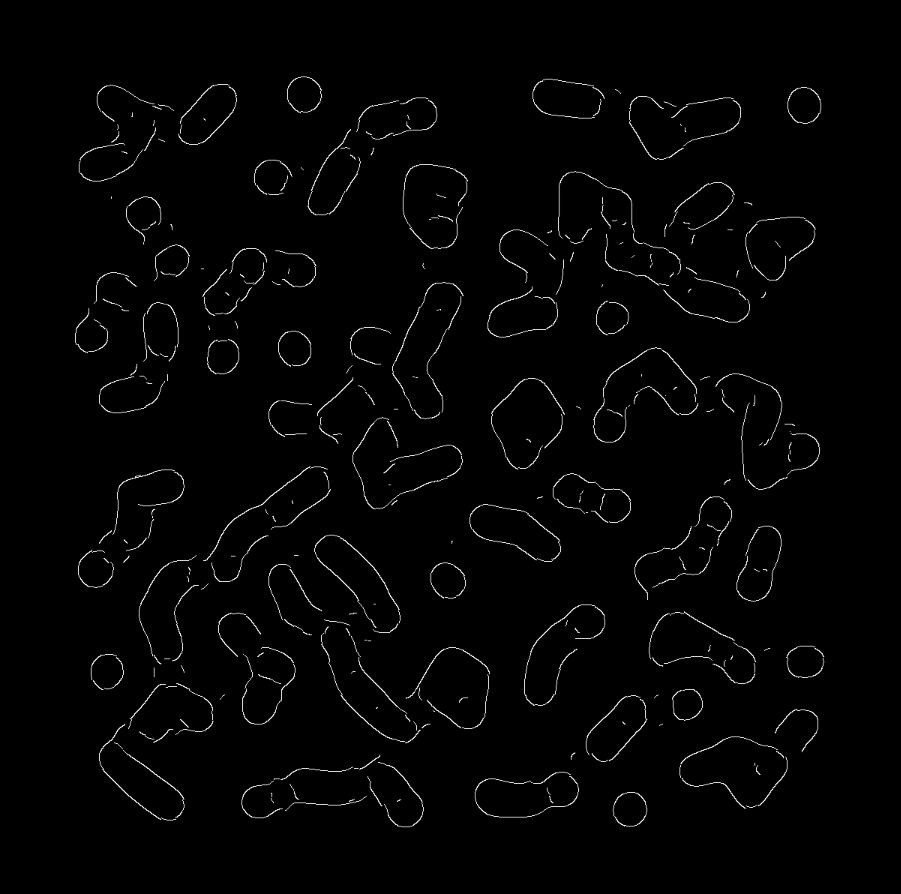
\includegraphics[width=0.3\textwidth]{latex-template-ss24/images/20_50_20_canny.png}
    \caption{Canny Edge Detection with Sigma: 20.0, Upper Threshold: 50\%, Lower Threshold: 20\%}
    \label{fig:20_50_20_canny}
\end{figure}

\textbf{Explanation:} At an extremely high Sigma value of 20.0, the image is heavily blurred, which greatly reduces noise but also results in the loss of most fine details. The very high thresholds (50\% upper and 20\% lower) ensure that only the strongest and most pronounced edges are detected. This configuration may be useful for applications where only the most critical edges need to be identified, but it risks overlooking important details in images with complex structures.

As observed in the generated images, increasing the Sigma value enhances the smoothing effect, which reduces noise but also risks losing finer details. Similarly, higher threshold values lead to fewer detected edges, focusing only on the most prominent features in the image. Selecting appropriate values for these parameters is crucial and should be tailored to the specific requirements of the edge detection task.
and edge detection requirements.


% \begin{table}[]
%     \centering
%     \begin{tabular}{l|c|c|c|c|c}
%         a & b & c & d & e & f \\
%     \hline
%         1 & 2 &0.2&0.3&0.4&0.5
%     \end{tabular}
%     \caption{In case you need a table.}
%     \label{tab:my_label}
% \end{table}

\newpage
\section{Conclusion}

In this project, we explored various image processing and thresholding techniques, applying them to enhance the clarity and visibility of images, which is crucial for medical imaging and other fields that rely on accurate image interpretation. Through our work, we demonstrated the importance of selecting the appropriate technique based on the specific requirements of the task at hand.

The basic thresholding methods, while straightforward and effective in simple scenarios, showed limitations when dealing with images with varying illumination or complex backgrounds. Advanced techniques such as Otsu's method provided better results in bimodal histograms by automatically determining the optimal threshold. However, even these methods can struggle with noisy images or those without clear intensity separation.

Edge detection techniques like Sobel, Scharr, and Prewitt provided more detailed insights into image boundaries, but they also exhibited sensitivity to noise and varying lighting conditions. The Canny Edge Detector, with its built-in noise reduction and double thresholding, proved superior for detecting edges with greater accuracy and reliability.

The work conducted in this project highlights the continuous trade-off between complexity and performance in image processing. Simple techniques are fast and easy to implement but may fail in challenging scenarios, while more sophisticated methods offer better results but require more computational resources and careful parameter tuning.

Two of the significant trends in the field of image processing are the application of deep learning techniques for image segmentation and the development of AI-based diagnostic tools.

1. \textbf{Deep Learning for Image Segmentation}: Convolutional Neural Networks (CNNs) and more advanced architectures like U-Net have become increasingly popular for image segmentation tasks, especially in medical imaging. These methods are capable of learning complex features directly from the data, enabling more accurate and robust segmentation even in challenging scenarios such as those involving noisy or low-contrast images \cite{Ronneberger2015Bio}. While deep learning-based segmentation is not yet fully integrated into clinical practice, it shows great promise due to its high accuracy and ability to generalize across different datasets.

2. \textbf{AI-Based Diagnostic Tools}: The integration of AI in diagnostic tools, such as those using deep learning for detecting diseases in radiology images, is another growing trend. These tools can assist radiologists by automatically highlighting areas of concern, potentially improving diagnostic accuracy and efficiency. Although these tools are increasingly being adopted in clinical settings, widespread implementation is still ongoing due to the need for extensive validation and the requirement for regulatory approval \cite{Esteva2017}.

Talking with respect to clinical, While deep learning for image segmentation is still largely in the research phase, with ongoing trials and validations, AI-based diagnostic tools are gradually being integrated into clinical workflows. The speed and accuracy these tools offer make them highly appealing, but challenges such as the need for large annotated datasets and the need to ensure their reliability across diverse patient populations must be addressed before they can be fully relied upon in clinical practice.

For the Future, the techniques implemented in the project showed varying degrees of success depending on the complexity of the image data. Simple methods like basic thresholding struggled with complex backgrounds and varying illumination, while advanced methods like Otsu's thresholding and the Canny Edge Detector performed better but still had limitations in terms of noise sensitivity and parameter dependence.

Future work could focus on integrating machine learning techniques to adaptively select parameters or even replace traditional methods with deep learning models that can automatically learn the best features for processing. Additionally, increasing the robustness of these techniques through better noise handling and improved generalization across different types of images could significantly enhance their practical applicability.

In conclusion, the project has provided a solid foundation in image processing techniques, highlighting both their potential and their limitations. With ongoing advancements in machine learning and AI, the future of image processing, particularly in medical diagnostics, looks promising.




% Literaturverzeichnis
\newpage
\bibliographystyle{apalike}
\bibliography{Bib/literatur}

\end{document}
  